\section{Результаты}

В эксперименте использована установка, состоящая из трубки с пористой перегородкой, через которую пропускается углекислый газ. Газ поступает в трубку через змеевик, расположенный в термостате, для поддержания постоянной начальной температуры газа. Трубка с перегородкой расположена в теплоизолированной трубе Дьюара.

Более подробное описание экспериментальной установки см. в \nameref{Приложение 1}.

Давление газа в трубке измеряется манометром. Манометр измеряет разность давлений в трубе и наружным (атмосферным). Так как второй конец трубки находится в области атмосферного давления, то манометр показывает перепад давления $-\Delta P$ на входе и выходе из трубки.

Разность $\Delta T$ температур газа на входе и выходе из трубки измеряется с помощью термопары, подключенной к цифровому мультиметру. Подробное описание способа определения $\Delta T$ по показаниям мультиметра см. в \nameref{Приложение 2}.

Температура $T$ углекислого газа на входе в трубку устанавливается с помощью контроллера термостата. Газ, текущий через змеевик, обменивается энергией с водой внутри термостата и нагревается до нужной температуры.

Каждая серия измерений зависимости $\Delta T(\Delta P)$ при новой температуре $T$ была проведена спустя промежуток времени в 5-7 минут после открытия вентиля трубы, чтобы минимизировать тепловые потери из-за обмена энергией между углекислым газом и трубкой. Когда достигнуто стационарное состояние и трубка нагрелась до температуры поступающего в нее газа, теплообмен между ними прекращается.

По измеренным зависимостям $\Delta T(\Delta P)$ (результаты в таблицах 2, 3, 4, 5, см. \nameref{Приложение 3}) для четырех различных температур $T$ построены графики. Результаты представлены на рисунке \ref{figure1}.
\begin{center}
    \label{figure1}
    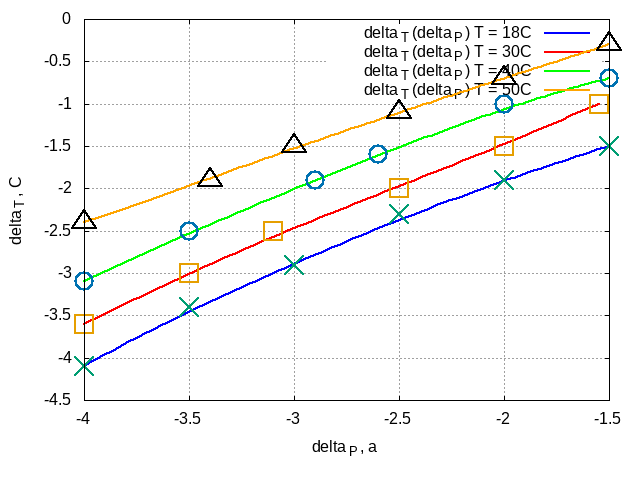
\includegraphics[width=0.9\textwidth]{img/graph6 (2).png}

    
    Графики зависимости разности $\Delta T$ температур газа на концах трубки от разности $\Delta P$ давлений газа на выходе из трубки и входе в нее при различных начальных температурах $T$ газа.
\end{center}



График зависимости $\Delta T(\Delta P)$ является линейным. При увеличении давления газа, поступающего в трубку, $\Delta T$ уменьшается. Чем больше давление газа, тем большую работу нужно совершить против сил притяжения молекул, чтобы удалить их на расстояние при расширении. Из этого следует, что больше становится потенциальная энергия газа и меньше - кинетическая. Так как кинетическая энергия пропорциональна температуре газа, то газ охлаждается до более низких температур.

По методу наименьших квадратов определены коэффициенты $\mu_\text{д-т}$ наклона прямых. Таблица значений $\mu_\text{д-т}$ при различных $T$ представлена в \nameref{Приложение 4}.

Используя данные из таблицы 6 (см. \nameref{Приложение 4}), построили график зависимости $\mu_{\text{д-т}}(T^{-1})$. 

\begin{figure}[ht]
\centering
    \begin{gnuplot}[terminal=pdf]
        set xlabel "1000/T"
        set ylabel "mu*10^{6}"
        set grid
        set key autotitle columnhead
        set pointsize 3

        f1(x) = a1*x + b1
        a1 = 1
        b1 = 1

        # Фитирование с вашими данными
        fit f1(x) "xxx" using ($1*1e3):($2*1e6) via a1, b1

        # Изображение данных и фитированной функции
        plot "xxx" using ($1*1e3):($2*1e6) smooth bezier title "μ(T^{-1})" with lines lw 2 lc "blue",\
             "xxx" using ($1*1e3):($2*1e6):($3*1e6):($4*1e6) with xyerrorbars title "Данные с погрешностями" pt -1 lc "red"
    \end{gnuplot}
    \caption{Графики зависимости $\mu_{\text{д-т}}(T^{-1})$. $\mu_{\text{д-т}}$ - коэффициент Джоуля-Томсона для углекислого газа, $\frac{1000}{T}$ - обратная температура газа, поступающего в трубку.}
    
\end{figure}


По методу наименьших квадратов и выражению \eqref{eq: mu} определены коэффициенты $a, b$. Результаты в Таблице 7 (см. \nameref{Приложение 5}).

Из выражения \eqref{eq: T_inv} определена инвариантная температура для углекислого газа
\[ T_{\text{инв}} = (571 \pm 93)K\]

Коэффициенты $a, b$ и температура $T_{\text{инв}}$ инверсии углекислого газа не совпадают с табличными (см. \nameref{Приложение 5}). Из этого следует, что модель газа Ван-дер-Ваальса подходит для качественного описания физических процессов, но не является достаточно точной для вычисления количественных характеристик системы.
